\documentclass[11pt]{article}

\usepackage[utf8]{inputenc}
\usepackage[T1]{fontenc}
%\RequirePackage{lmodern}	% font set: Latin Modern
\RequirePackage{charter}	% font set: Charter

\usepackage[french,english]{babel}

% Package ADDED
\usepackage{xcolor,graphics,graphicx}

% For citations
\usepackage{csquotes}

% For line spacing
\usepackage{setspace}
\linespread{1.3}

% To rotate a table or a figure
\usepackage{lscape}
% MATHS
% To manage cells in table
\newcommand{\tabcell}[2][c]{%
	\begin{tabular}[#1]{@{}l@{}}#2\end{tabular}}

%% The amssymb package provides various useful mathematical symbols
\usepackage{amssymb}
\usepackage{amsmath}
\usepackage{empheq}

% TAILLE de la page
\usepackage{geometry} % define page margin
\geometry{top=20mm,left=30mm,right=30mm,bottom=20mm} % margin from top, left, right and bottom

% COMPTEUR de ligne
%% The lineno packages adds line numbers. Start line numbering with
%% \begin{linenumbers}, end it with \end{linenumbers}. Or switch it on
%% for the whole article with \linenumbers after \end{frontmatter}.
\usepackage{caption}
\usepackage{lineno}
\linenumbers

% BIBLIOGRAPHIE
%\usepackage[numbers]{natbib}
\usepackage[authoryear]{natbib}
\usepackage{hyperref}

\begin{document}


% USED TO ADD "S" in front of Table, Figure, Equation
\setcounter{table}{0}
\renewcommand{\thetable}{S\arabic{table}}%
\setcounter{figure}{0}
\renewcommand{\thefigure}{S\arabic{figure}}%
\setcounter{equation}{0}
\renewcommand{\theequation}{S\arabic{equation}}%

% ------------- TITLE PAGE

\begin{center}
	\huge\textbf{
	Supporting Information
	}\par
\end{center}

\begin{center}
	\Large\textbf{
		Trophic transfer of anticoagulant rodenticides while managing rodent pests: the fine line between predator-prey regulation and pesticide-pest regulation
	}\par
\end{center}

\vspace{.5cm}

\begin{center}
	\large\textbf{
		Virgile Baudrot$^{1,2}$ 
		Javier Fernandez-de-Simon$^{1,3}$
		Michael Coeurdassier$^1$,
		Geoffroy Couval$^{1,4}$,
		Patrick Giraudoux$^1$,
		Xavier Lambin$^{5,6}$		
	}\par	
\end{center}
~\\
$^1$ Université Bourgogne Franche-Comté - UMR CNRS 6249 Laboratoire Chrono-environnement, 25030 Besançon, France\\
$^2$ BioSP, INRA, 84000 Avignon, France\\
$^3$ IREC. Instituto de Investigación en Recursos Cinegéticos\\
$^4$ FREDON Franche-Comté, Espace Valentin Est, 12, Rue de Franche-Comté - Bât E, 25480 Ecole-Valentin, France\\
$^5$ School of Biological Sciences, University of Aberdeen, Zoology Building, Tillydrone Avenue, Aberdeen AB24 2TZ, Scotland, UK\\
~\\
$^*$ Corresponding authors: virgile.baudrot@posteo.net or x.lambin@abdn.ac.uk


 \clearpage

% -----------------------------

\section{Model derivation}


% GRAPHIC SCHEME

\begin{figure}[!htb]
	\begin{center}
		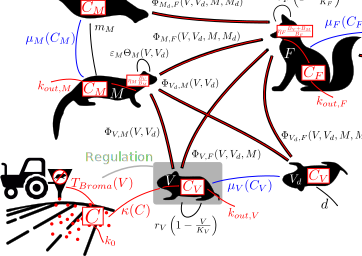
\includegraphics[width=.8\linewidth]{img/system_scheme.png}
		\caption{Dynamics of mustelids (bold grey line) and red foxes (bold black line) after 50 years of simulation (10 years of burn-in period, shaded area, and 40 years considered here for the compute of results, estimation of 
			cost functions, etc.). Letters at the top-right part of each sub-graph corresponds to the results obtained from each farmer functional response. FR (dashed line) and MR (dotted line) indicate the farmer-regulated and mustelid-regulated periods of vole population dynamics.}
		\label{fig:scheme}
	\end{center}
\end{figure}


\subsection{Dynamic of populations for the tri-trophic dynamic}
%
The population dynamics of a tri-trophic system is commonly described as follow:
\begin{equation}
\left\{
\begin{array}{l l}
\dfrac{dV}{dt} & =  r_V V \left( 1- \dfrac{V}{K_V}\right) - \Phi_{V,M}(V)M - \Phi_{V,F}(V,M)F\\[.3cm]
%
\dfrac{dM}{dt} & = \varepsilon_M B_V \Phi_{V,M}(V)M - m_M M - \Phi_{M,F}(V,M)F\\[.3cm]
%
\dfrac{dF}{dt} & = F r_F \left( 1- \dfrac{F}{K_F}\right)
\end{array}
\right.
\label{eq:simpleSystem}
\end{equation}

As described in the manuscript, the vole population, $V$ followed a logistic growth rate, with $r_V$  the maximal reproduction rate, fixed at $r_V = \ln(2 \times 600)/365$ in [day$^{-1}$], since montane water vole populations can increase from 0  to  600 individuals ha$^{-1}$ or more in a year \citep{Giraudoux1997} resulting in the equilibrium density being fixed at $K_V = 600$ individuals.
%
Other variable and parameters are detailed hereafter.

\subsubsection{About the logistic model}

The idea behind this parametrization is the use of a classical Malthusian equation with $r_V$ in [day$^{-1}$] and $V$ in [ind ha$^{-1}$]:

\begin{equation}
\frac{dV}{dt} = r_V V \quad \Rightarrow \quad
V(t) = V(0) \exp(r_V t) \quad \Rightarrow \quad
r_V = \ln\left( \frac{V(t)}{V(0)} \right) \times \frac{1}{t}
\end{equation}
So to have the maximal growth rate $r_V$, we need the greatest $V(t)$ (measured at 600 ind ha$^{-1}$ but supposed to be more in theoretical optimal condition) obtained in the minimum of time (less than a year). 
%
Then, to add the carrying capacity $K_V$ in [ind$^{-1}$], we use the logistic equation and assumed the carrying capacity to be the one measured in the environment:
\begin{equation}
\frac{dV}{dt} = r_V V \left( 1 - \frac{V}{K_V}\right)
\end{equation}


The estimation of $r$ using the Malthusian function and then applying the carrying capacity $K$ can be seen as non consistent because of the dependency of $r_V$ to $K_V$. 
%
For isntance, in \citet{Ginzburg1992}, the author says that going from $dV/dt = r_V V$ to $dV/dt = r_V V (1-V/K_V)$ would be correct if $r$ was independent of resource limitation $K_V$:

\textit{"Two populations  of a species live in environments  identical in all  respects, that is, they  have the same resource availability  and any  other imaginable characteristics. One of the two is subject to  higher mortality. There is no doubt  that the population growth curves in these two cases will be different. Are the final equilibrium abundances different? Most ecologists will answer that the equilibrium values should be the same and that the higher rate of reproduction just means that the population will ‘get there faster’, but reach the same level nevertheless".}


Then, \citet{Ginzburg1992} states that their is two ways to reflect the extra mortality: either assuming (a) $dV/dt = r_V V(1-V/K_V) - mV$ or (b) $dV/dt = (r_V-m_V)V(1-V/K_V)$.
%
In equation (a), the equilibirum depend on $r$: $V^* = (r_V-m_V) K_V /r_V$, so is wrong with the un-changed equilibrium assumption.
%
And re-writing (b) gives: $dV/dt = rV(1-V/K_V) - m_V V(1-V/K_V)$. Since $- m_V V(1-V/K_V)$ reflects an environmental pressure, it should not be positive when $V>K_V$. Meaning, when the population is over it’s carrying capacity, we are going to growth even faster and to infinity.
%
In the present manuscript, we made assumption (a), and we assume that $r$ is not independent of resource limitation $K_V$. It is for instance well known that vole reproduction rate is linked to the state of resource at the time of reproduction \citep{Pinot2016}.


Many authors respond to Ginzburg \citep{Olson1992, Watkinson1992, Mackenzie1992, Berryman1992} and later \citep{Gabriel2005}.  

In his response, \citet{Olson1992} says: \textit{“While the logistic model is often defined as non-mechanistic, it has the attractive feature of describing population growth with only two parameters, $K$ and $r$. $K$ is universally defined as the population-carrying capacity. However, there is much disagreement about the definition of  $r$ and this disagreement has affected conclusions derived from the use of the logistic equation.”}
%
\citet{Olson1992} suggests that the problem is the intuition assigned to the r-independence to equilibirum density $K$.
%
Again in our line, \citet{Watkinson1992} argues that \textit{"Most ecologists, he asserts, would believe that the equilibrium values of these two populations should be the same. In that case I must be one of the minority who does not believe this to be so."} 

Another answer by \citet{Berryman1992} proposed to rewrite the model in order to see the link between $r$ and $K$. The approach by \citet{Berryman1992} is interesting as it introduces a relevant effect of considering  the exploitation rate (link to the growth rate) within the carrying capacity, meaning a carrying capacity with its on dynamic (e.g., with its resilience depending on how exploitation happen), and non an extra-system static one.

\subsubsection{Predation of voles, and predator dynamics}

The vole population was preyed upon by mustelid and fox populations, denoted $M$ and $F$ respectively in \eqref{eq:simpleSystem}. The vole consumption rate at different vole densities was described by functional responses ($\Phi_{V,M}$ for mustelids, $\Phi_{V,F}$  for foxes).

\begin{equation}
\begin{array}{l l}
\Phi_{V,M}(V) = \dfrac{a_M V}{1 + h_M a_M V} \\[.3cm]
%
\Phi_{V,F}(V) = \dfrac{a_{VF} V}{a_{VF}V + a_{MF}F} \times \dfrac{(a_{VF}V + a_{MF} M)^2}{1 + h_F(a_{VF}V + a_{MF} M)^2}\\[.3cm]
%
\Phi_{M,F}(V,M) = \dfrac{a_{MF}V}{a_{VF}V + a_{MF}F} \times \dfrac{(a_{VF}V + a_{MF}M)^2}{1+h_F(a_{VF}V + a_{MF}M)^2}
\end{array}
\label{eq:functionResponse}
\end{equation}


We treated small mustelids as vole specialist predators \citep{King2006}, assuming a Holling Type 2 functional response with attack rate $a_M$ in [day$^-1$] and handling time $h_M$ in [day] (equation \eqref{eq:functionResponse}). We then represented foxes feeding on voles and mustelids by a multi-species functional response derived from Holling Type 3, referring to generalist feeding behaviour \citep{Baudrot2016}. For that, we denoted $a_{VF}$ and $a_{MF}$ (both in  [day$^-1$]) the fox attack rate on voles and mustelids respectively. The parameter $h_F$ was the handling time for foxes in [day].

Consequently, the functional responses $\Phi_{X,Y}$ are all in [day$^{-1}$].  And the functions:
 
$\dfrac{dV}{dt}  =  r_V V \left( 1- \dfrac{V}{K_V}\right) - \Phi_{V,M}(V)M - \Phi_{V,F}(V,M)F$ and $\dfrac{dF}{dt} = F r_F \left( 1- \dfrac{F}{K_F}\right)$ are also consistent, all part being in [ind ha$^{-1}$ day$^{-1}$].


\subsubsection{Conversion efficiency and mortality rate in mustelid population}

The parameterization of the conversion efficiency of ingested food into new born, $\varepsilon_M B_V$ (the parameter $B_V$ is the constant mean biomass of one individual as we explain latter, but could be integrated into a general constant parameter since $B_V$ is a constant) in [n.d.] (non dimensional, so with $B_V$ in [kg], in this formulation $\varepsilon_M$ is in [kg$ {-1}$], which is a rate by kg), and the mortality rate, $m_M$ in [day$^{-1}$], in equation \eqref{eq:simpleSystem} is not straightforward since we have to take into account the mortality rate due to starvation.
% 
In the situation of no starvation, ageing, diseases and predation of mustelids are the main reason of death. In the situation of no prey availability at initial condition, then the mortality rate of mustelids should be equal to the mortality rate without food. 
Using the simplest scheme of Dynamic Energy Budget (DEB) theory (seeFigure~\ref{fig:DEB_scheme}), the ingested food is assimilated for a part, we denote $\alpha$ and non-assimilated for another part, $(1- \alpha)$. Then, the assimilated part goes to a reserve (or directly use) in either the somatic maintenance or in the maturity maintenance (to produce reproductive tools). In DEB, a proportion $\kappa$ from the reserve is the part allocated to somatic maintenance [n.d.] and a proportion $1-\kappa$ is addressed to the maturity maintenance.


\begin{figure}[!htb]
	\begin{center}
		\includegraphics[width=.5\linewidth]{img/DEB_scheme.png}
		\caption{Representation of the standard dynamic energy budget (DEB model \citep{Sousa2010}}
		\label{fig:DEB_scheme}
	\end{center}
\end{figure}

Figure~\ref{fig:DEB_scheme} represents the standard dynamic energy budget (DEB) model \citep{Sousa2010}.
%
Then, assuming the generic functional response $\Phi_{V,M}(V)$, the reproduction rate of the predator is like:
\begin{equation}
\Phi_{V,M}(V) \alpha (1 - \kappa) \varepsilon'
\end{equation}
where $\varepsilon'$ in [n.d.] is the conversion efficiency of daily assimilated food for one individual, dedicated for reproduction into newborn mustelids.

Then, $\alpha \kappa \Phi_{V,M}$ is the part allocated to somatic maintenance structure. Parameters $\alpha$ and $\kappa$ are non-dimensional [n.d.].

We can then take into account the starvation process in the mortality rate, with a food-independent mortality rate $m_{M, -\Phi}$ in [day$^{-1}$] and a part depending on food availability $m_{M, +\Phi} = \sigma \alpha \kappa \Phi_{V,M}$ in [day$^{-1}$], with $\sigma$ [n.d.] a conversion parameter.


Then, the dynamic of Mustelid given in the manuscript equation \eqref{eq:simpleSystem} could be rewritten as:
\begin{equation}
\frac{dM}{dt} = \Phi_{V,M}(V) \alpha (1 - \kappa) \varepsilon' M - \left( m_{M, -\Phi}  + \sigma \alpha \kappa \Phi_{V,M} \right) M - \Phi_{M,F}(V, M) F
\end{equation}

Which is equal to:
\begin{equation}
\frac{dM}{dt} = \left(\alpha (1 - \kappa) \varepsilon' - \sigma \alpha \kappa  \right) \Phi_{V,M}(V)  M - m_{M, -\Phi}  M  - \Phi_{M,F}(V, M) F
\end{equation}

Therefore, if we set  the food-independent mortality rate $m_M = m_{M, -\Phi}$ and the conversion efficiency of ingested food $\varepsilon_M B_V=\alpha ((1 - \kappa) \varepsilon' - \sigma  \kappa ) $ , we get back to the equation provided in model \eqref{eq:simpleSystem} but with a clearer definition of $\varepsilon_M B_V$.

This is why we parameterized $m_M$ in [day$^{-1}$] as the inverse of life expectancy in [day$^{-1}$], and $\varepsilon_M B_V$ in [n.d.] as an unclear parameter derived from the null model (i.e., without AR) to reflect observed population dynamics. 

In any case, the dimension of the equation
\begin{equation}
\dfrac{dM}{dt}  = \varepsilon_M B_V \Phi_{V,M}(V)M - m_M M - \Phi_{M,F}(V,M)F
\label{eq:dynamic_M}
\end{equation}
%
is well defined, since $\varepsilon_M B_V \Phi_{V,M}(V)$ is in [day$^{-1}$].

\subsection{Dynamic of populations with AR}

After spreading by farmer, in the model AR is degraded or transferred to voles, which are exposed to the environmental contaminant mainly through ingestion of contaminated foodstuffs (i.e., trophic transfer), and AR accumulates in their tissues and is release with rate $k_{out,V}$.
%
Contaminants in an individual, the body burden, are commonly measured in concentration per mass of individual, [$\mu$g g$^{-1}$ ind$^{-1}$] (equivalent to [mg kg$^{-1}$ ind$^{-1}$] and denoted [ppm ind$^{-1}$]).
%
Predators are only exposed to contaminant through the consumption of voles, a trophic transfer, so as a function of functional response.
\\


To consider both toxicological and population dynamics within the same equation, we convert population dynamics into dynamics of their biomasses as in \citep{Huang2015EcoTox, Baudrot2018}.

We denote $V$, $V_d$ $M$, $F$ the densities of voles, dead voles, mustelids and foxes respectively ; $B_V$, $B_{V_d}$, $B_M$ and $B_F$ the mean biomass of an individual of those species in [g ind$^{-1}$], and $B_{T,V}$, $B_{T,V_d}$, $B_{T,M}$ and $B_{T,F}$ the total biomass of the population in the space unit we used, so in [g ha$^{-1}$]. In other words, $B_{T,X} = B_X \times X$. The notation $C_V$, $C_{V_d}$ $C_M$ and $C_F$ holds for the mean concentration of the contaminant in one individual, commonly called the body burden of the prey in ppm [mg kg$^{-1}$].
%
The growth function of the prey population is a function $g_X(X, \zeta_X)$ in [day$^{-1}$] depending on the population density $X$ and the dose of the contaminant $\zeta_X$, either the internal concentration $C_X$ or the dose eaten $D_X$.
%
The dose-response curve $\mu_X(\zeta_X)$ is defined by a log-normal cumulative distribution function as in \cite{Loos2010}.


\paragraph{Variables for the population dynamics}
%
To convert individual dynamics into biomass dynamics, we just multiplied the variable density $X$ in [ind ha$^{-1}$] with a constant $B_X$ in [g ind$^{-1}$], so that the derivative as just to be multiplied by this constant: 
%
\begin{equation}
\frac{d B_{T,X}}{dt} = \frac{d B_X X}{dt} = B_X \frac{d X}{dt} \quad \text{and so we have} \quad  \frac{d X}{dt} = \frac{1}{B_X} \times \frac{d B_{T,X}}{dt}
\label{eq:biomTOpop}
\end{equation}
%

\subsubsection{Dynamic of the contaminant in the environment}

In the agro-ecotoxico-logical system, we consider an environmental concentration of contaminant denoted by $w_{ext}$ in [mg ha$^{-1}$] in order to reflect the spatially explicit spreading of AR following determined in baits per area.
%
From the Figure~\ref{fig:scheme}, we can directly provide the dynamic of this concentration:


\begin{equation}
\frac{dw_{ext}}{dt} = T_{Broma}(V) - k_0w_{ext} - \kappa(w_{ext})V B_V
\end{equation}

with $T_{Broma}(V)$ the farmer input of AR in [mg ha$^{-1}$ day$^{-1}$] depending on vole density denoted $V$ in [ind ha$^{-1}$].
%
AR concentration in baits is 50 $\mu$g g$^{-1}$ (or mg kg$^{-1}$). So when farmer spread in grasslands at quantity 7.5 to 20 kg ha$^{-1}$ day$^{-1}$, its an amount of 375 to 1000 mg ha$^{-1}$ of AR spread (i.e., mg kg$^{-1}$ $\times$ kg ha$^{-1}$ day$^{-1}$ ).


The disappearance of AR in the field, denoted $k_0$, in [day$^{-1}$], so that $k_0 w_{ext}$ is in [mg ha$^{-1}$ day$^{-1}$].
%
Such quantity, $w_{ext}$, was available in the literature, and a proportion disappeared in the environment at rate $k_0 = 0.0815$ day$^{-1}$ \citep{Sage2008}.


The function $\kappa(w_{ext})$, in [mg kg$^{-1}$ day$^{-1}$], reflects the transfer of contaminant from the environmental compartment to the vole compartment. As a consequence, the term $\kappa(w_{ext})V B_V$ is in [mg ha$^{-1}$ day$^{-1}$] ([mg kg$^{-1}$ day$^{-1}$] $\times$ [kg ha$^{-1}$]).


This rate $\kappa(w_{ext})$ was assumed to be an increasing function characterized by a maximum intake rate $M_{in}$ in [mg kg$^{-1}$ day$^{-1}$], and a half-saturation constant for ingestion $D_{in}$ in [mg ha$^{-1}$] since $w_{ext}$ is in [mg ha$^{-1}$]:

\begin{equation}
\kappa(w_{ext})= M_{in}\times \dfrac{ w_{ext}}{D_{in} + w_{ext}}
\end{equation}

So the dimension of the ingestion rate $\kappa(w_{ext})$ is the same as $M_{in}$ that is [mg kg$^{-1}$ day$^{-1}$].


\subsubsection{The dose in dose-response}

The dose of the dose-response function can be either based on the exposure in the environment, the food ingested or the internal concentration. While data used in this paper are considering internal concentration for voles, this is the ingested concentration used for mustelids and predators.

For the dynamic of dose, we consider an homogeneous population, where the dose eaten, or the internal concentration are equal to all individuals within a population. We denote $\zeta_X$ such a dose.

\paragraph{Dynamic of the dose eaten: $\zeta_X$}
%
Since predators are only exposed to the contaminant through the functional response, we introduce $D_{V,M}$, $D_{V,F}$ and $D_{M,F}$  which are respectively the doses of contaminant include in food of individuals in [$\mu$g g$^{-1}$ day$^{-1}$ ind$^{-1}$].
%
For simplification of writing, we write $D_M = D_{V,M}$ and $D_F = D_{V,F}+D_{M,F}$
%
Since $D_X$ it is by kg of the predator $X$, we have to take into account variation of the biomass of this predator already defined by $B_{T,X}$. Therefore we first define the total amount of contaminant eaten by mustelids $w_{exp,M}$ in [mg pop$_M^{-1}$ or mg ha$^{-1}$] and derive the dose.
%
\begin{equation}
w_{exp,X} = D_X B_X X = D_X B_{T,X} \quad \Rightarrow \quad \frac{dw_{exp,X}}{dt} = B_X \frac{dX D_X}{dt} = B_X \left( X \frac{dD_X}{dt} + D_X \frac{dX}{dt} \right)
\end{equation}
%
Therefore, $\dfrac{dw_{exp,X}}{dt}$ is in [mg pop$^{-1}$ day$^{-1}$] or, since we consider a close population within one ha, it is in  [mg ha$^{-1}$ day$^{-1}$].

Also:
%
\begin{equation}
\frac{dD_X}{dt} = \frac{dw_{exp,X}/B_{T,X}}{dt} = \dfrac{1}{B^2_{T,X}} \left( B_{T,X} \frac{dw_{exp,X}}{dt} + w_{exp,X} \frac{dB_{T,X}}{dt} \right)
\end{equation}
%

\paragraph{Dynamic of the internal concentration}
%
As for the dose provided, we set a new variable $w_X = C_X B_X X$ which is in [$\mu$g g$^{-1}$] $\times$ [g ind$^{-1}$] $\times$ [ind ha$^{-1}$], so that:
%
$w_X$ is in [mg ha$^{-1}$] or [mg population$^{-1}$], which is the quantity of contaminant within the population.
%
The dynamic of the new variable is defined with:
%
\begin{equation}
w_X = C_X B_X X = C_X B_{T,X} \quad \Rightarrow \quad \frac{dw_X}{dt} = B_X \frac{dX C_X}{dt} = B_X \left( X \frac{dC_X}{dt} + C_X \frac{dX}{dt} \right)
\end{equation}
%
and $\dfrac{dw_X}{dt}$ is in [mg ha$^{-1}$ day$^{-1}$].
%



\subsubsection{Dynamics of contaminant within populations}

With all the assumptions made in the manuscript, especially the assumption that individuals of a same population have the same biomass and the same amount of contaminant in their bodies, the model for the transfer of a contaminant  is given by:
%

\begin{subequations}
	\begin{empheq}[left={\empheqlbrace\,}]{align}
	% OUTSIDE toxic
	\dfrac{dw_{ext}}{dt} & =  T_{Broma}(V) - k_0w_{ext} - \kappa(w_{ext})B_{T,V} 
	\label{eq:General_Mod:a} \\[3mm]
	% VOLE Dynamic
	\dfrac{dB_{T,V}}{dt} & = 
	B_{T,V} r_V\left( 1- \dfrac{V}{K_V} \right)	- \mu_V(\zeta_V)B_{T,V} -  B_V (\Phi_{V,M}(V) M - \Phi_{V,F}(V,M) F)
	\label{eq:General_Mod:b} \\[3mm]
	% VOLE toxic
	\dfrac{dw_{V}}{dt} & = \kappa(w_{ext}) B_{T,V} - w_V(k_{out, V} + \mu(\zeta_V)) - \notag\\[3mm]
	&  C_V B_V ( \Phi_{V,M}(V)M + \Phi_{V,F}(V,M)F )
	\label{eq:General_Mod:c} \\[3mm]
	%
	% MUSTELID dynamic
	\dfrac{dB_{T,M}}{dt} & = 
	B_{T,M} (\varepsilon_MB_V  \Phi_{V,M}(V) - m_M - \mu_M(\zeta_M) ) - B_M \Phi_{M,F}(V, M) F
	\label{eq:General_Mod:d} \\[3mm]
	% MUSTELID toxic
	\dfrac{dw_{M}}{dt} & =  - k_{out, M} w_M - w_M (m_M + \mu_M(\zeta_M))  - C_M B_M \Phi_{M,F}(V,M)F   + \notag \\[3mm]
	&  \eta_M C_V B_V \Phi_{V,M}(V)M 
	\label{eq:General_Mod:e} \\[3mm]
	%
	% FOX dynamic
	\dfrac{dB_{T,F}}{dt} & = 
	B_{T,F} r_F\left( 1- \dfrac{F}{K_F} \right)	- \mu_F(\zeta_F) B_{T,F}
	\label{eq:General_Mod:f}  \\[3mm]
	% FOX toxic
	\dfrac{dw_{F}}{dt} & =  - k_{out, F} w_F - w_F \mu_F(\zeta_F) + \notag \\[3mm]
	& \eta_F \left( C_V B_V \Phi_{V,F}(V,M) F +  C_M B_M \Phi_{M,F}(V,M) F\right)  
	\label{eq:General_Mod:g}
	\end{empheq}
	\label{eq:General_Mod}
\end{subequations}

In the general model \eqref{eq:General_Mod}, the equations \eqref{eq:General_Mod:b}, \eqref{eq:General_Mod:d} and \eqref{eq:General_Mod:f} present the dynamic of the total biomass of voles, mustelids and foxes respectively.
%
The equations \eqref{eq:General_Mod:a}, \eqref{eq:General_Mod:c}, \eqref{eq:General_Mod:e} and \eqref{eq:General_Mod:g} stand for the dynamics of contaminant concentrations in the environment and within individuals for respectively the voles, mustelids and foxes. The parameter $k_{out,X}$ is the excretion rate of the contaminant and the death of individuals implies a decrease of amounts of the contaminant, respectively $ -w_X m_X$ and $-w_X \mu_X(\zeta_X)$ with $\zeta_X$ being either the internal concentration $C_X$ or the dose eaten $D_X$. For predators, data provide a dose-response mortality function resulting from a the ingestion dose and not the internal concentration.
%
The transfer of the contaminant through the predation is express by the term $ C_X B_X \Phi(X)Y$, which is removed in prey contaminant dynamic $w_X$ and added in the predator contaminant dynamic $w_Y$ (with a factor of transfer efficiency $\eta_Y$).
%


While we could consider the population dynamic in term of biomasses, it is more convenient to use density of population as suggested by the change of variables which are as follows:

\paragraph{Internal concentration}~\\

\begin{enumerate}
	\item Conversion of the dynamics of biomass of population, $B_{T,X}$ into dynamics of the density, $X$. From the equation \eqref{eq:biomTOpop}, we have: $\dfrac{d B_{T,X}}{dt} = B_X \dfrac{d X}{dt}$
	\item Conversion of amount of contaminant, $w_X$, into within population concentration, $C_X$:	
	$$\dfrac{d C_X}{dt}  = \dfrac{d w_X / B_{T,X}}{dt} = \dfrac{1}{B_{T,X}^2} \left( \dfrac{d w_X}{dt} B_{T,X} - w_X \dfrac{d B_{T,X}}{dt}\right)$$
\end{enumerate}

Using these properties, we can convert part of system \eqref{eq:General_Mod}:


\begin{equation}
\left\lbrace
\begin{array}{c c l}
\dfrac{dC_V}{dt} & = & \dfrac{d w_V / B_{T,V}}{dt} = \dfrac{1}{B_{T,V}^2} \left( \dfrac{d w_V}{dt} B_{T,V} - w_V\dfrac{d B_{T,V}}{d t}\right) \\[3mm]
%
& = & \dfrac{1}{B_{T,V}} \left(\kappa(w_{ext})B_{T,V} - k_{out,V}w_V - w_V \mu_V(C_V) - C_V B_V(\Phi_{V,M}(V)M + \Phi_{V,F}(V,M)F ) \right) - \\[3mm]
& & \dfrac{w_V}{B_{T,V}^2} \left( B_{T,V} g_V{V,C_V} - \mu_V(C_V) B_{T,V} - B_V(\Phi_{V,M}(V)M + \Phi_{V,F}(V,M)F \right)  \\[3mm]
%
& = & \kappa(w_{ext}) - C_V \left( k_{out,V} + r_V\left( 1- \dfrac{V}{K_V} \right)\right)
\end{array}
\right.
\end{equation}


%
\begin{equation}
\left\lbrace
\begin{array}{c c l}
\dfrac{dC_M}{dt} & = & \dfrac{d w_M / B_{T,M}}{dt} = \dfrac{1}{B_{T,M}^2} \left( \frac{d w_M}{d t} B_{T,M} - w_M \frac{dB_{T,M}}{dt} \right)\\[3mm]
%
& = & \dfrac{B_{T,M}}{B_{T,M}^2} \left[ - k_{out,M} w_M - w_M(m_M + \mu_M(D_M)) + \eta_M C_V B_V \Phi_{V,M}(V)  - C_M B_M \Phi_{M,F}(V,M)F \right] - \\[3mm]
& &\dfrac{w_M}{B_{T,M}^2]} \left[ B_{T,M} (\varepsilon_M B_V \Phi_{V,M}(V) - m_M - \mu_M(D_M) ) - B_M \Phi_{M,F}(V,M)F  \right]\\[3mm]
%
& = &\dfrac{1}{B_{T,M}} \left[ C_M B_{T,M} (- k_{out,M} - m_M - \mu_M(D_M)- \Phi_{M,F}(V,M)F) + \eta_M C_V B_V \Phi_{V,M}(V)M  \right]  -  \\[3mm]
&  & C_M(\varepsilon_M B_V \Phi_{V,M}(V) - m_M - \mu_M(D_M)) + \frac{B_M}{B_{T,M}} C_M \Phi_{M,F}(V,M)F\\[3mm]
%
& = & C_M(-k_{out,M} - m_M - \mu_M(D_M)) + \dfrac{1}{B_{T,M}} \eta_M C_V B_V \Phi_{V,M}(V)M - \Phi_{M,F}(V,M)F - \\[3mm]
&  & C_M \varepsilon_M B_V \Phi_{V,M}(V) + C_M(m_M + \mu_M(D_M) + \Phi_{M,F}(F)F \\[3mm]
%
& = & \eta_M C_V \dfrac{B_V}{B_M} \Phi_{V,M}(V) - C_M \left( k_{out,M} + \varepsilon_M B_V \Phi_{V,M}(V)\right)
\end{array}
\right.
\end{equation}


\begin{equation}
\left\lbrace
\begin{array}{c c l}
\dfrac{d C_F}{dt} & = & \dfrac{d w_F / B_{T,F}}{dt} = \dfrac{1}{B_{T,F}^2} \left( \dfrac{d w_F}{dt} B_{T,F} - w_F \dfrac{d B_{T;F}}{dt}\right) \\[3mm]
%
& = & \dfrac{1}{B_{T,F}} \left( - k_{out,F}w_F - w_F \mu_F(D_F) + \eta_F(C_M B_M \Phi_{M,F}(V,M)F + C_V B_V \Phi_{V,F}(V,M)F) \right) - \\[3mm] 
& & \dfrac{w_F}{B_{T,F}^2} \left( B_{T,F} r_F\left( 1- \dfrac{F}{K_F} \right) - B_{T,F} \mu_F(D_F) \right) \\[3mm]
%
& = & \eta_F \left( C_V \dfrac{B_V}{B_F} \Phi_{V,F}(V,M) + C_M \dfrac{B_M}{B_F} \Phi_{M,F}(V,M)  \right) - C_F \left( k_{out,F} + r_F\left( 1 - \dfrac{F}{K_F} \right)\right) 
\end{array}
\right.
\end{equation}


%
In addition, for dead voles, we assume the following dynamics:

\begin{equation}
\dfrac{dB_{T,V_d}}{dt}  = \mu_V(C_V)B_{T,V}
\end{equation}

and

\begin{equation}
\dfrac{dw_{V_d}}{dt}  = \dfrac{dw_{V}}{dt}
\end{equation}
%


\paragraph{Dose ingested}~\\
As for internal concentration, we first define the total amount of contaminant eaten by population $X$ $w_{exp,X}$ in [mg pop$_X^{-1}$ day$^{-1}$ or mg ha$^{-1}$ day$^{-1}$] and derive the dose as:

\begin{equation}
\left\lbrace
\begin{array}{c  l}
\dfrac{dD_M}{dt} & =  \dfrac{d w_{exp,M} / B_{T,M}}{dt} = \dfrac{1}{B_{T,M}^2} \left(\dfrac{d w_{exp,M}}{dt} B_{T,M} - \dfrac{d B_{T,M}}{dt} w_{exp,M}\right)
\\[3mm]
%
& =  \dfrac{1}{B_{T,M}} C_V B_V \Phi_{V,M}(V)M - \\[3mm]
& \dfrac{D_M B_{T,M}}{B_{T,M}^2} \left( 	B_{T,M} (\varepsilon_MB_V  \Phi_{V,M}(V) - m_M - \mu_M(D_M) ) - B_M \Phi_{M,F}(V, M) F \right)	\\[3mm]
& =  \dfrac{C_V B_V \Phi_{V,M}(V)}{B_M} - D_M	(\varepsilon_MB_V  \Phi_{V,M}(V) - m_M - \mu_M(D_M) ) + \dfrac{D_M \Phi_{M,F}(V, M) F}{M}  	
\end{array}
\right.
\end{equation}


And, with the same approach for foxes:

\begin{equation}
\left\lbrace
\begin{array}{c  l}
\dfrac{dD_F}{dt} & =  \dfrac{d w_{exp,F} / B_{T,F}}{dt} = \dfrac{1}{B_{T,F}^2} \left(\dfrac{d w_{exp,F}}{dt} B_{T,F} - \dfrac{d B_{T,F}}{dt} w_{exp,F}\right)
\\[3mm]
%
& =  \dfrac{1}{F B_F} (C_V B_V \Phi_{V,F}(V,M)F + C_M B_M \Phi_{M,F}(V,M)F ) - \\[3mm]
& \dfrac{D_F }{B_{T,F}} \left( 	B_{T,F} r_F\left( 1- \dfrac{F}{K_F} \right)	- \mu_F(D_F) B_{T,F}\right)	\\[3mm]
& =  \dfrac{C_V B_V \Phi_{V,F}(V,M) + C_M B_M \Phi_{M,F}(V,M)}{B_F} -  D_F \left(r_F \left( 1- \dfrac{F}{K_F} \right)	- \mu_F(D_F)  \right)	
\end{array}
\right.
\end{equation}

\paragraph{General model}~\\

As a consequence of all these assumptions, the model as implemented for simulations is given by:

\begin{equation}
\left\lbrace
\begin{array}{c c l}
% VOLE Dynamic
\dfrac{dV}{dt} & = &
\overbrace{	r_V V \left( 1- \dfrac{V}{K_V} \right)		}^{\text{growth rate}} -
\overbrace{	\mu_V(C_V)V	}^{\text{poisoning}} -
\overbrace{	\Phi_{V,M}(V,V_d)M - \Phi_{V,F}(V,V_d,M)F	}^{\text{predation}}\\[3mm]
%
% DEAD VOLE Dynamic
\dfrac{dV_d}{dt} & = &
\overbrace{ \mu_V(C_V)V }^{\text{new dead voles}} -
\overbrace{	\Phi_{V_d,M}(V,V_d)M - \Phi_{V_d,F}(V,V_d,M)F	}^{\text{predation}}-
\overbrace{d V_d}^{\text{degradation}}
\\[3mm]
%
% MUSTELIDS Dynamic
\dfrac{dM}{dt} & = &
\overbrace{	(\varepsilon_M B_V \Theta_M(V,V_d)-m_M) M	}^{\text{growth rate}} - 
\overbrace{\mu_M(D_M)M	}^{\text{poisoning}} -
\overbrace{\Phi_{M,F}(V,V_d,M)F }^{\text{predation}} \\[3mm]
%
% F0X Dynamic
\dfrac{dF}{dt} & = &
\overbrace{	r_F F (1-F/K_F)	}^{\text{growth rate}} -
\overbrace{\mu_F(D_F)F	}^{\text{poisoning}}  \\
%
%
% Toxicological dynamics
\dfrac{dw_{ext}}{d t}  & = & 
\overbrace{T_{Broma}(V)}^{\text{treatment}} - 
\overbrace{k_0 w_{ext}}^{\text{degradation}} -
\overbrace{\kappa(w_{ext}) V}^{\text{consumption}} \\[3mm]
%
% Toxico-kinetics in Voles
\dfrac{dC_V}{dt} & = &
\overbrace{\kappa(C)}^{\text{intake}} - 
\overbrace{C_V\left(k_{out,V} + r_V \left(1 - \dfrac{V}{K_V}\right)\right)}^{\text{excretion}}\\[3mm]
%
% Toxico-kinetics in Mustelids
\dfrac{dC_M}{d t} & = &
\overbrace{\eta_M \dfrac{B_V}{B_M} (\Phi_{V,M}(V,V_d,M)+\Phi_{V_d,M}(V,V_d,M)) C_V}^{\text{intake}} -
\overbrace{C_M\left(k_{out,M} + \varepsilon_M B_V \Phi_{V,M}(V,V_d,M) \right)}^{\text{excretion}} \\[3mm]
%
\dfrac{dD_M}{d t} & = &
\overbrace{
\dfrac{ B_V }{B_M}C_V\Phi_{V,M}(V)}^{\text{exposure}}
\overbrace{ - D_M \left(\varepsilon_MB_V  \Phi_{V,M}(V)
 - m_M - \mu_M(D_M) -\Phi_{M,F}(V, M) \dfrac{F}{M} \right)}^{\text{population change}}   \\[3mm]
%
% Toxico-kinetics in Foxes
\dfrac{dC_F}{d t} & = &
\overbrace{ \eta_F  \left( \dfrac{B_V}{B_F} (\Phi_{V,M}(V,V_d,M)+\Phi_{V_d,M}(V,V_d,M)) C_V + \dfrac{B_M}{B_F}\Phi_{M,F}(V,V_d,M) C_M \right)}^{\text{intake}} - \\[3mm]
& &
\overbrace{C_F \left( k_{out,F} + r_F \left(1 - \dfrac{F}{K_F}\right) \right) }^{\text{excretion}}  \\[3mm]
\dfrac{dD_F}{d t} & = &
\overbrace{
 \dfrac{C_V B_V \Phi_{V,F}(V,M) + C_M B_M \Phi_{M,F}(V,M)}{B_F} }^{\text{exposure}} 
\overbrace{ - D_F \left(r_F \left( 1- \dfrac{F}{K_F} \right)	- \mu_F(D_F)  \right)	}^{\text{population change}}
\end{array}
\right.
\label{eq:Sys_complet}
\end{equation}

 \clearpage

\section{Additional results of simulations}

\subsection{Results with Foxes}

\begin{figure}[!htb]
	\begin{center}
		\includegraphics[width=\linewidth]{img/graph_0_0.png}
		\caption{Variation of population densities and contaminant concentration in soil simulated over 50 years. Scenario \textbf{a}: 0 AR. Variables are: $D.F$ for fox density, $D.M$ for mustelid density, $D.V$ for vole density, $D.Vd$ for dead vole density and $C.soil$ for AR concentration in the environment.}
	\end{center}
\end{figure}

\begin{figure}[!htb]
	\begin{center}
		\includegraphics[width=\linewidth]{img/graph_500_20.png}
		\caption{Variation of population densities and contaminant concentration in soil simulated over 50 years. Scenario \textbf{b}: threshold 500 in ha$^{-1}$ and 20 kg ha$^-1$ of AR.  Variables are: $D.F$ for fox density, $D.M$ for mustelid density, $D.V$ for vole density, $D.Vd$ for dead vole density and $C.soil$ for AR concentration in the environment.}
	\end{center}
\end{figure}

\begin{figure}[!htb]
	\begin{center}
		\includegraphics[width=\linewidth]{img/graph_250_20.png}
		\caption{Variation of population densities and contaminant concentration in soil simulated over 50 years. Scenario \textbf{c}: threshold 250 in ha$^{-1}$ and 20 kg ha$^-1$ of AR. Variables are: $D.F$ for fox density, $D.M$ for mustelid density, $D.V$ for vole density, $D.Vd$ for dead vole density and $C.soil$ for AR concentration in the environment.}
	\end{center}
\end{figure}

\begin{figure}[!htb]
	\begin{center}
		\includegraphics[width=\linewidth]{img/graph_250_7_5.png}
		\caption{Variation of population densities and contaminant concentration in soil simulated over 50 years. Scenario \textbf{d}: threshold 250 in ha$^{-1}$ and 7.5 kg ha$^-1$ of AR. Variables are: $D.F$ for fox density, $D.M$ for mustelid density, $D.V$ for vole density, $D.Vd$ for dead vole density and $C.soil$ for AR concentration in the environment.}
	\end{center}
\end{figure}

\begin{figure}[!htb]
	\begin{center}
		\includegraphics[width=\linewidth]{img/graph_50_7_5.png}
		\caption{Variation of population densities and contaminant concentration in soil simulated over 50 years. Scenario \textbf{e}: threshold 50 in ha$^{-1}$ and 7.5 kg ha$^-1$ of AR. Variables are: $D.F$ for fox density, $D.M$ for mustelid density, $D.V$ for vole density, $D.Vd$ for dead vole density and $C.soil$ for AR concentration in the environment.}
	\end{center}
\end{figure}

\begin{figure}[!htb]
	\begin{center}
		\includegraphics[width=\linewidth]{img/plt_sobolIndex_0_0.png}
		\caption{First-order Sobol's sensitivity index. Scenario \textbf{a}: No AR.}
	\end{center}
\end{figure}


\begin{figure}[!htb]
	\begin{center}
		\includegraphics[width=\linewidth]{img/plt_sobolIndex_500_20.png}
		\caption{First-order Sobol's sensitivity index. Scenario \textbf{b}: threshold 500 voles in ha$^{-1}$ and 20 kg ha$^-1$ of AR.}
	\end{center}
\end{figure}


\begin{figure}[!htb]
	\begin{center}
		\includegraphics[width=\linewidth]{img/plt_sobolIndex_250_20.png}
		\caption{First-order Sobol's sensitivity index. Scenario \textbf{c}: threshold 250 voles in ha$^{-1}$ and 20 kg ha$^-1$ of AR.}
	\end{center}
\end{figure}


\begin{figure}[!htb]
	\begin{center}
		\includegraphics[width=\linewidth]{img/plt_sobolIndex_250_7_5.png}
		\caption{First-order Sobol's sensitivity index. Scenario \textbf{d}: threshold 250 voles in ha$^{-1}$ and 7.5 kg ha$^-1$ of AR.}
	\end{center}
\end{figure}


\begin{figure}[!htb]
	\begin{center}
		\includegraphics[width=\linewidth]{img/plt_sobolIndex_50_7_5.png}
		\caption{First-order Sobol's sensitivity index. Scenario \textbf{e}: threshold 50 voles in ha$^{-1}$ and 7.5 kg ha$^-1$ of AR.}
	\end{center}
\end{figure}

 \clearpage

\subsection{Results without Foxes}

\begin{table}[!htb]
	\caption{Results on the cost functions for the comparison of treatment protocols. Column \textit{"FFR"} (farmer functional response) refers to the protocol denotation (a to e) and in brackets respectively: the vole density threshold, and the amount of AR/treatment in kg. The column \textit{"Nbr treat/yr"} refers to the number of treatment in simulation per year after the burn-in phase. \textit{"Total AR/yr"} is the total use of anticoagulant rodenticides per year (bromadiolone in kg). \textit{"M, 50\% AR death"} is the proportion of time with mortality by AR over 50\% in mustelids population. \textit{"M, 50\% Nat. death"} is the proportion of time with mortality by natural reason (i.e., all except AR) over 50\% in mustelids population. \textit{"V < 50 ha$^{-1}$"} is the proportion of time with less than 50 voles ha$^{-1}$. Finally, \textit{"Mean V density"}, \textit{"Mean M density"} and \textit{"Mean F density"} are mean densities of voles, mustelids and foxes respectively.}	
	\label{tab:SMresults}
	\begin{tabular}{p{2cm} c c c c c c c c}
		\hline
		\tabcell{FFR \\ (dose, limit)} &
		\tabcell{Nbr. \\ treat/yr} &
		\tabcell{Total  \\ AR/yr} &
		\tabcell{M, 50\% \\ AR death} &
		\tabcell{M, 50\% \\ Nat. death} &
		\tabcell{V < \\ 50 ha$^{-1}$} &
		\tabcell{Mean V \\ density} & 
		\tabcell{Mean M \\ density} & 
		\tabcell{Mean F \\ density} \\
		\hline
		%%
		a (0,0)    & 0& 0& 0& 1& 0.5               & 215 & 0.61   & 0\\
		% 
		b (500,20) & 4.4& 88 & 0.03 &0.97 & 0.4     & 185 & 0.57 & 0\\
		%
		c (250, 20) & 2.3 & 46 &0.06 & 0.93 & 0.2 & 110 & 0.31 & 0\\
		%
		d (250, 7.5)& 4.9 & 37 & 0.04 & 0.96 & 0.3 & 116 & 0.58 & 0\\
		%
		e (50,7.5) & 5.6 &  42 & 0 & 1 & 0.9   & 55 & 0.08 & 0 \\
		\hline
	\end{tabular}
\end{table}

\begin{figure}[!htb]
	\begin{center}
		\includegraphics[width=\linewidth]{img/plot_join_0F.png}
		\caption{Rate of variation of population densities simulated over 50 years (10 years of burn-in period in grey area): (Left) Dynamics of mustelids (grey line) and red foxes (black line), (Right) Dynamics of live (grey line) and dead (black line) voles. Letters at the top-center part of each sub-graph corresponds to the results obtained from each farmer functional response. Red area and Green area indicate the farmer-regulated (FR) and mustelid-regulated (MR) periods of vole population dynamics respectively.}
		\label{fig:populations}
	\end{center}
\end{figure}

\begin{figure}[!htb]
	\begin{center}
		\includegraphics[width=\linewidth]{img/graph_0_0_0F.png}
		\caption{Variation of population densities and contaminant concentration in soil simulated over 50 years. Scenario \textbf{a}: 0 AR. Variables are: $D.F$ for fox density, $D.M$ for mustelid density, $D.V$ for vole density, $D.Vd$ for dead vole density and $C.soil$ for AR concentration in the environment.}
	\end{center}
\end{figure}

\begin{figure}[!htb]
	\begin{center}
		\includegraphics[width=\linewidth]{img/graph_500_20_0F.png}
		\caption{Variation of population densities and contaminant concentration in soil simulated over 50 years. Scenario \textbf{b}: threshold 500 in ha$^{-1}$ and 20 kg ha$^-1$ of AR. Variables are: $D.F$ for fox density, $D.M$ for mustelid density, $D.V$ for vole density, $D.Vd$ for dead vole density and $C.soil$ for AR concentration in the environment.}
	\end{center}
\end{figure}

\begin{figure}[!htb]
	\begin{center}
		\includegraphics[width=\linewidth]{img/graph_250_20_0F.png}
		\caption{Variation of population densities and contaminant concentration in soil simulated over 50 years. Scenario \textbf{c}: threshold 250 in ha$^{-1}$ and 20 kg ha$^-1$ of AR. Variables are: $D.F$ for fox density, $D.M$ for mustelid density, $D.V$ for vole density, $D.Vd$ for dead vole density and $C.soil$ for AR concentration in the environment.}
	\end{center}
\end{figure}

\begin{figure}[!htb]
	\begin{center}
		\includegraphics[width=\linewidth]{img/graph_250_7_5_0F.png}
		\caption{Variation of population densities and contaminant concentration in soil simulated over 50 years. Scenario \textbf{d}: threshold 250 in ha$^{-1}$ and 7.5 kg ha$^-1$ of AR. Variables are: $D.F$ for fox density, $D.M$ for mustelid density, $D.V$ for vole density, $D.Vd$ for dead vole density and $C.soil$ for AR concentration in the environment.}
	\end{center}
\end{figure}

\begin{figure}[!htb]
	\begin{center}
		\includegraphics[width=\linewidth]{img/graph_50_7_5_0F.png}
		\caption{Variation of population densities and contaminant concentration in soil simulated over 50 years. Scenario \textbf{e}: threshold 50 in ha$^{-1}$ and 7.5 kg ha$^-1$ of AR. Variables are: $D.F$ for fox density, $D.M$ for mustelid density, $D.V$ for vole density, $D.Vd$ for dead vole density and $C.soil$ for AR concentration in the environment.}
	\end{center}
\end{figure}


% BIBLIOGRAPHY
% \section*{References}

 \clearpage

\bibliographystyle{elsarticle-harv}
%\bibliographystyle{plainnat}
%\bibliographystyle{unsrt}
\bibliography{trophToxNTO.bib}



\end{document}
